\documentclass[portuguese]{artigo}
\newcommand\x{\mathrm{x}}
\newcommand\D{\vetor{\x} - \vetor{\x'}}
\author{Louis Bergamo Radial\\8992822}
\title{Eletromagnetismo - 4302303\\Lista de Exercícios VIII}
\begin{document}
   \maketitle
   \setcounter{tcb@cnt@exercício}{1}
   % \begin{exercício}{Campo magnético de um fio longo com ângulo reto}{exercício1}
    Um fio muito longo carrega uma corrente estacionária \(I\) e faz uma curva de ângulo reto como abaixo. Calcule o campo magnético no ponto \(P\) indicado em cada uma das duas situações indicadas.
    \begin{center}
        \begin{tikzpicture}[scale=0.7,every node/.style={scale=0.7}]
            \node at (1,-2.5) {Situação (a)};
            \draw[thick] (0,-2) -- (0,0);
            \draw[thick, -stealth] (0,-2) -- (0,-1);
            \draw[thick, -stealth] (0,0) -- (1,0) node[above] {\(I\)};
            \draw[thick] (0,0) -- (2,0);
            \filldraw[thick] (0, 1) circle(0.01) node[anchor=west] {\(P\)};
            \draw[dotted] (0,0) -- (0,1) node[midway,anchor=east] {\(d\)};
            \begin{scope}[xshift=7cm]
                \node at (1,-2.5) {Situação (b)};
                \draw[thick] (0,-2) -- (0,0);
                \draw[thick, -stealth] (0,-2) -- (0,-1);
                \draw[thick, -stealth] (0,0) -- (1,0) node[above] {\(I\)};
                \draw[thick] (0,0) -- (2,0);
                \filldraw[thick] +(135:1) circle(0.01) node[anchor=south] {\(P\)};
                \draw[dotted] (0,0) -- +(135:1) node[midway,anchor=north] {\(d\)};
                \draw[dotted] (0,0) -- +(315:0.5);
                \draw[thick] (0.5,0) arc[start angle=360, end angle=315, radius=0.5]  node[anchor=west] {\(\frac{\pi}{4}\)};
            \end{scope}
        \end{tikzpicture}
    \end{center}
\end{exercício}
\begin{proof}[Resolução]
    Consideremos um ponto \(\vetor{\x} = d(\cos\varphi \vetor{e}_x + \sin\varphi \vetor{e}_y)\), então pela lei de Biot-Savart temos
    \begin{align*}
        \vetor{B}(\vetor{\x}) &= \frac{\mu_0I}{4\pi} \left[\int_{-\infty}^0\dli{y} \frac{\vetor{e}_y \times (\vetor{\x} -y\vetor{e}_y)}{\norm{\vetor{\x} - y\vetor{e}_y}^{\frac32}} + \int_{0}^\infty \dli{x}\frac{\vetor{e}_x \times (\vetor{\x} - x\vetor{e}_x)}{\norm{\vetor{\x} - x\vetor{e}_x}^{\frac32}}\right]\\
                              &= \frac{\mu_0 I d}{4\pi} \left\{-\int_{-\infty}^0\dli{y}\frac{\cos\varphi}{\left[(y - d\sin\varphi)^2 + d^2\cos^2\varphi\right]^{\frac32}} + \int_0^\infty\dli{x} \frac{\sin\varphi}{\left[(x - d\cos\varphi)^2 + d^2 \sin^2\varphi\right]^{\frac32}}\right\}\vetor{e}_z.
    \end{align*}
    Assim, segue que
    \begin{equation*}
        \vetor{B}(\vetor{\x}_{\mathrm{(a)}}) = \frac{\mu_0 I d}{4\pi} \int_0^\infty\dli{x}\frac{1}{(x^2 + d^2)^{\frac32}} = \frac{\mu_0 I d}{4\pi}\left[\int_{0}^{\frac{\pi}{2}}\dli{\theta} \frac{\cos\theta}{d^2}\right] \vetor{e}_z= \frac{\mu_0 I}{4\pi d} \vetor{e}_z
    \end{equation*}
    e
    \begin{align*}
        \vetor{B}(\vetor{\x}_\mathrm{(b)}) &= \frac{\mu_0 I d}{4\pi\sqrt{2}} \left\{\int_{-\infty}^0\dli{y}\left[\left(y - \frac{d}{\sqrt{2}}\right)^2 + \frac{d^2}{2}\right]^{-\frac32} + \int_0^{\infty}\dli{x}\left[\left(x + \frac{d}{\sqrt{2}}\right)^2 + \frac{d^2}{2}\right]^{-\frac32}\right\}\vetor{e}_z\\
                                           &= \frac{\mu_0 I d}{4\pi\sqrt{2}} \left\{\int_0^{\infty}\dli{\tilde{y}}\left[\left(\tilde{y} + \frac{d}{\sqrt{2}}\right)^2 + \frac{d^2}{2}\right]^{-\frac32} + \int_0^{\infty}\dli{x}\left[\left(x + \frac{d}{\sqrt{2}}\right)^2 + \frac{d^2}{2}\right]^{-\frac32}\right\}\vetor{e}_z\\
                                           &= \frac{\mu_0 I d}{2\pi \sqrt{2}} \left(\int_{\frac\pi4}^{\frac\pi2}\dli{\theta} \frac{\cos\theta}{\frac{d^2}{2}}\right)\vetor{e}_z\\
                                           &= \frac{\mu_0 I}{\pi \sqrt{2}d} \left(1 - \frac{1}{\sqrt{2}}\right)\vetor{e}_z
    \end{align*}
    são as expressões do campo magnético nos pontos das duas situações.
\end{proof}

   \begin{exercício}{Condições de contorno para meios lineares}{exercício2}
    Na interface entre dois meios dielétricos, o campo elétrico deve necessariamente ser consistente com as condições de contorno que você resumiu no problema anterior. Assim, considere uma interface genérica entre dois meios \emph{lineares}, como mostra a figura abaixo. As constantes \(\epsilon_1\) e \(\epsilon_2\) correspondem às permissividades elétricas de cada um dos meios e os campos elétricos estão indicados.

    \begin{center}
        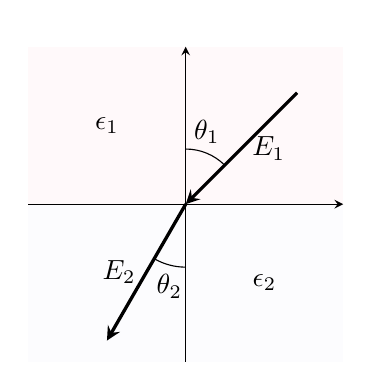
\begin{tikzpicture}
            \fill[Lavender!10] (-2,-2) rectangle (2,0);
            \fill[Pink!10] (-2,0) rectangle (2,2);
            % Axes
            \draw[-stealth] (-2,0) -- (2,0) node[right] {};
            \draw[-stealth] (0,-2) -- (0,2) node[above] {};

            % Arrows for E1 and E2 using polar coordinates
            \draw[very thick, stealth-] (0,0) -- +(45:2) node[midway,right] {$\vetor{E}_1$};
            \draw[very thick, -stealth] (0,0) -- +(-120:2) node[midway,left] {$\vetor{E}_2$};

            % Theta1 angle
            \draw (0,0.7) arc[start angle=90,end angle=45,radius=0.7] node[midway,above] {\(\theta_1\)};

            % Theta2 angle
            \draw (0,-0.8) arc[start angle=270,end angle=240,radius=0.8] node[midway, below] {\(\theta_2\)};

            % Labels for permittivities
            \node at (-1,1) {$\epsilon_1$};
            \node at (1,-1) {$\epsilon_2$};
        \end{tikzpicture}
    \end{center}

    Prove que \(\epsilon_2 \tan{\theta_1} = \epsilon_1 \tan{\theta_2}\).
\end{exercício}
\begin{proof}[Resolução]

\end{proof}

   % \begin{exercício}{Dipolo magnético na presença de um campo uniforme}{exercício4}
    Em uma região do espaço encontra-se um campo magnético uniforme, \(\vetor{B}_0 = B_0 \vetor{e}_z\). Adicionalmente, um dipolo magnético do tipo \(\vetor{m} = -m_0 \vetor{e}_z\), com \(m_0 > 0\), é colocado na origem do sistema de coordenadas. Mostre que existe uma superfície esférica, centrada na origem pela qual não passam linhas de campo magnético. Encontre o raio dessa esfera e faça um esboço das linhas de campo, internas e externas a essa superfície. Assuma que o campo magnético gerado pelo dipolo é dado pela expressão do problema anterior.
\end{exercício}
\begin{proof}[Resolução]
    Pelo \cref{ex:exercício3}, o campo total é dado por
    \begin{equation*}
        \vetor{B}(\vetor{\x}) = B_0 \vetor{e}_z + \frac{\mu_0}{4\pi \norm{\vetor{\x}}^5} \left[3 \inner{\vetor{\x}}{\vetor{m}}\vetor{\x} - \norm{\vetor{\x}}^2 \vetor{m}\right] = \left(B_0+\frac{\mu_0m_0}{4\pi \norm{\vetor{\x}}^3}\right)\vetor{e}_z - \frac{3\mu_0\inner{\vetor{\x}}{\vetor{e}_z}m_0 \vetor{\x}}{4\pi \norm{\vetor{\x}}^5}.
    \end{equation*}
    Assim, o fluxo de campo magnético pela superfície esférica \(\Omega_R\) de raio \(R\) centrada na origem é
    \begin{align*}
        \Phi(R) = \int_{\Omega_R} \dln3\x \vetor{n} \cdot \vetor{B}(\vetor{\x})
        &= \int_{0}^{\pi} R \dli{\theta} \int_0^{2\pi}R \sin\theta \dli{\varphi} \left[\left(B_0 + \frac{\mu_0 m_0}{4\pi R^3}\right) \cos\theta - \frac{3\mu_0m_0 \cos\theta}{4\pi R^3}\right]\\
        &= \frac{1}{2R} \int_0^\pi \sin\theta \dli{\theta} \left[4\pi R^3 B_0 - 2\mu_0 m_0\right]\cos\theta\\
        &= \frac{1}{2R} \left(4\pi R^3 B_0 - 2\mu_0 m_0\right).
    \end{align*}
    Dessa forma, para \(R_0 = \left(\frac{\mu_0 m_0}{2\pi B_0}\right)^{\frac13}\), temos \(\Phi(R_0) = 0\).

    \todo[Linhas de campo.]
\end{proof}

   % \begin{exercício}{Energia de interação entre dois dipolos magnéticos ideais}{exercício5}
    Mostre que a energia de interação entre dois dipolos magnéticos ideais \(\vetor{m}_1\) e \(\vetor{m}_2\) pode ser escrita como
    \begin{equation*}
        U = \frac{\mu_0}{4\pi \norm{\vetor{\x}_2 - \vetor{\x}_1}^3}\left[\inner{\vetor{m}_1}{\vetor{m}_2} - 3\inner*{\vetor{m}_1}{\frac{\vetor{\x}_2 - \vetor{\x}_1}{\norm{\vetor{\x}_2 - \vetor{\x}_1}}}\inner*{\vetor{m}_2}{\frac{\vetor{\x}_2 - \vetor{\x}_1}{\norm{\vetor{\x}_2 - \vetor{\x}_1}}}\right]
    \end{equation*}
    em que \(\vetor{\x}_i\) é a posição do dipolo de momento \(\vetor{m}_i\).
\end{exercício}
\begin{proof}[Resolução]

\end{proof}

   % \begin{exercício}{Cabo coaxial}{exercício6}
    Um cabo coaxial longo possui uma densidade volumétrica de carga uniforme \(\rho\), positiva, no cilindro interno (raio \(a\)), e uma densidade superficial de carga uniforme na casca externa do cilindro (raio \(b\)). Essa carga superficial é negativa e de magnitude exata para que o cabo, como um todo, seja eletricamente neutro.
    \begin{center}
        \includegraphics[width=0.4\linewidth]{exercício06.png}
    \end{center}
    \begin{enumerate}[label=(\alph*)]
        \item Encontre o campo elétrico em todo o espaço (onde ele é bem definido), e escreva a densidade superficial de carga em \(s = b\) em termos de \(\rho,\) \(a\) e \(b\). Faça um gráfico da intensidade do campo elétrico em função de \(s\).
        \item Encontre agora o potencial elétrico em todo o espaço, assumindo que \(\phi(s = 0) = \phi_0\). Em particular, indique o valor da diferença de potencial \(\phi(b) - \phi(a)\).
        \item Calcule a energia eletrostática armazenada na configuração por unidade de comprimento do cabo.
\end{enumerate}
\end{exercício}
\begin{proof}[Resolução]
    Utilizemos um sistema de coordenadas cilíndricas coaxial ao eixo de simetria do cabo. Seja
    \begin{equation*}
        \varrho(\vetor{\x}) = \begin{cases}
            \rho,&\text{se }s \leq a\\
            \sigma \delta(s - b),&\text{se }s > a
        \end{cases}
    \end{equation*}
    a distribuição volumétrica de cargas do cabo coaxial, onde \(\sigma\) é a densidade superficial na casca cilíndrica de raio \(b\). Seja \(\family{\Omega_R}{R \in \mathbb{R}^+} \subset \mathbb{R}^3\) uma família de volumes cilíndricos de altura \(h\) centrados na origem e coaxiais ao cabo, indexados pelo raio \(R > 0\). A carga total \(Q(R)\) contida no cilindro \(\Omega_R\) é dada por
    \begin{align*}
        Q(R) = \int_{\Omega_R}\dln3\x \varrho(\vetor{\x}),
    \end{align*}
    logo
    \begin{equation*}
        Q(R) = \begin{cases}
            \rho \pi h R^2, &\text{se }R \leq a\\
            \rho \pi h a^2, &\text{se }a < R < b\\
            \rho \pi h a^2 + 2 \pi b h\sigma, &\text{se }R > b,
        \end{cases}
    \end{equation*}
    como facilmente se constata. Para que o cabo seja neutro, devemos ter
    \begin{equation*}
        \sigma = -\frac{a^2}{2b}\rho,
    \end{equation*}
    de modo que \(Q(R) = 0\) para todo \(R \geq b\).

    Consideremos o potencial eletrostático \(\phi = \phi(s, \theta, z)\). Pela simetria de translação na direção do eixo do cabo e pela rotação ao redor deste eixo devemos ter
    \begin{equation*}
        \diffp{\phi}{z} = \diffp{\phi}{\theta} = 0,
    \end{equation*}
    donde segue que \(\phi = \phi(s)\). Concluímos, portanto, que o campo elétrico é dado por \(\vetor{E} = -\diffp{\phi}{s} \vetor{e}_s\), e podemos escrever \(\vetor{E} = E(s) \vetor{e}_s,\) onde \(E\) é a intensidade do campo.

    Pela lei de Gauss, temos
    \begin{equation*}
        \oint_{\partial \Omega_R} \vetor{E}\cdot \vetor{n} \dl{S} = \frac{1}{\epsilon_0} \int_{\Omega_R}\dln3\x \varrho(\vetor{\x}) \implies 2\pi R h E(R) = \frac{Q(R)}{\epsilon_0},
    \end{equation*}
    para todo \(R > 0\) com \(R \neq b\). Desse modo,
    \begin{equation*}
        E(R) = \begin{cases}
            \dfrac{\rho R}{2 \epsilon_0},&\text{se }R \leq a\\
            \dfrac{\rho a^2}{2 \epsilon_0 R}, &\text{se }a < R < b\\
            0,&\text{se }R > b
        \end{cases}
    \end{equation*}
    descreve a intensidade do campo elétrico em todo o espaço, exceto na casca cilíndrica \(R = b\). Isto é, o campo elétrico é dado por
    \begin{equation*}
        \vetor{E}(s \vetor{e}_s + z \vetor{e}_z) = \begin{cases}
            \dfrac{\rho s}{2 \epsilon_0}\vetor{e}_s,&\text{se }s \leq a\\
            \dfrac{\rho a^2}{2 \epsilon_0 s}\vetor{e}_s, &\text{se }a < s < b\\
            \vetor{0},&\text{se }s > b.
        \end{cases}
    \end{equation*}

    \begin{figure}[!ht]
        \centering
        \begin{tikzpicture}
            \begin{axis}[
                width=0.8\linewidth,
                height=0.2\textheight,
                xmin=0, xmax=4.1,
                ymin=-0.01,ymax=1.25,
                domain=0:5,
                samples=10000,
                axis lines=middle,
                xlabel={\(s\)},
                ylabel={\(\norm{\vetor{E}}\)},
                legend pos=north east,
                ytick={0,1/e,1},
                yticklabels={0,\(\frac{\rho a^2}{2 \epsilon_0 b}\), \(\frac{\rho a}{2 \epsilon_0}\)},
                xtick={0,1,e},
                xticklabels={0, \(a\), \(b\)},
                % grid=both,
                % grid style={line width=.1pt, draw=Surface0},
                % major grid style={line width=.2pt,draw=Overlay2},
                % minor tick num=3,
            ]
                \addplot[very thick, Mauve, jump mark left] {x < 1 ? x : (x < e ? 1/x : 0)};
                \draw[dotted] (axis cs:1,1) -- (axis cs:1,0);
                \draw[dashed, thick, Mauve] (axis cs:e,1/e) -- (axis cs:e,0);
                \addplot[dashed] {1};
                \addplot[dashed] {1/e};
            \end{axis}
        \end{tikzpicture}
        \caption{Intensidade do campo elétrico gerado por um cabo coaxial infinito para todo \(s \neq b\).}
    \end{figure}

    Seja \(\family{\Gamma_r}{r \in \mathbb{R}^+}\) uma família de caminhos simples e retilíneos que começam em algum ponto tal que do eixo de simetria \(s = 0\), com direção radial, indexados pela distância ao eixo do cabo \(s = r \in \mathbb{R}^+\) de seu ponto de término. O potencial \(\phi(r)\) em algum ponto no cilindro de raio \(r\) é, portanto,
    \begin{equation*}
        \phi(r)  = \phi_0 -\int_{\Gamma_r} \vetor{E}\cdot \dl{\vetor{\ell}}.
    \end{equation*}
    Para \(r \in [0, a)\), temos
    \begin{equation*}
        \phi(r) = \phi_0 -\int_{0}^{r} \dli{s} \frac{\rho s}{2 \epsilon_0}= \phi_0 - \frac{\rho r^2}{4 \epsilon_0},
    \end{equation*}
    e em particular vale \(\phi(a) = \phi_0 - \frac{\rho a^2}{4 \epsilon_0}\), por conta da continuidade do potencial. Para \(r \in [a, b)\), temos
    \begin{equation*}
        \phi(r) = \phi(a) - \int_a^r \dli{s}\frac{\rho a^2}{2 \epsilon_0 s} = \phi_0 - \frac{\rho a^2}{4 \epsilon_0} - \frac{\rho a^2}{2 \epsilon_0} \ln\left(\frac{r}{a}\right),
    \end{equation*}
    e concluímos \(\phi(b) = \phi_0 - \frac{\rho a^2}{4 \epsilon_0} - \frac{\rho a^2}{2 \epsilon_0}\ln\left(\frac{b}{a}\right)\) por continuidade. Para \(r > b\) segue que \(\phi(r) = \phi(b)\), uma vez que o campo elétrico se anula.

    \begin{figure}[!ht]
        \centering
        \begin{tikzpicture}
            \begin{axis}[
                width=0.8\linewidth,
                height=0.2\textheight,
                xmin=0, xmax=4.1,
                ymin=-0.01,ymax=1.85,
                domain=0:5,
                samples=10000,
                axis lines=middle,
                xlabel={\(s\)},
                ylabel={\phi(s) - \phi(b)},
                legend pos=north east,
                ytick={0,1,3/2},
                yticklabels={0,\(\frac{\rho a^2}{2 \epsilon_0}\ln\left(\frac{b}{a}\right)\), \(\frac{\rho^2}{4 \epsilon_0} + \frac{\rho a^2}{2 \epsilon_0}\ln\left(\frac{b}{a}\right)\)},
                xtick={0,1,e},
                xticklabels={0, \(a\), \(b\)},
                % grid=both,
                % grid style={line width=.1pt, draw=Surface0},
                % major grid style={line width=.2pt,draw=Overlay2},
                % minor tick num=3,
            ]
                \addplot[very thick, Mauve, jump mark left] {x < 1 ? 3/2 - x^2/2 : (x < e ? 1 - ln(x) : 0)};
                \draw[dotted, Mauve] (axis cs:1,1) -- (axis cs:1,0);
                \addplot[dashed] {3/2};
                \addplot[dashed] {1};
            \end{axis}
        \end{tikzpicture}
        \caption{Diferença de potencial elétrico em relação a \(\phi(b)\).}
    \end{figure}
    Isto é, o potencial é dado por
    \begin{equation*}
        \phi(s) = \begin{cases}
            \phi_0 - \dfrac{\rho s^2}{4 \epsilon_0}, &\text{se }s \in [0,a)\\
            \phi_0 - \dfrac{\rho a^2}{2 \epsilon_0}\left[\dfrac{1}{2} + \ln\left(\dfrac{s}{a}\right)\right], &\text{se }s\in[a,b]\\
            \phi_0 - \dfrac{\rho a^2}{2 \epsilon_0}\left[\dfrac{1}{2} + \ln\left(\dfrac{b}{a}\right)\right], &\text{se }s\in(b, \infty)
        \end{cases}
    \end{equation*}
    e em particular temos \(\phi(b) - \phi(a) = - \frac{\rho a^2}{2 \epsilon_0} \ln\left(\frac{b}{a}\right)\).

    A densidade de energia eletrostática armazenada na configuração é dada por
    \begin{equation*}
        u = \frac12 \epsilon_0 \norm{E}^2 = \begin{cases}
            \frac{\rho^2 s^2}{8\epsilon_0}, & \text{se }s \in [0, a]\\
            \frac{\rho^2 a^4}{8 \epsilon_0 s^2}, &\text{se }s \in (a, b)\\
            0, &\text{se }s \in (b, \infty).
        \end{cases}
    \end{equation*}
    Desse modo, a energia \(U_{\ell}\) armazenada em um volume \(\Sigma_\ell = \setc*{\vetor{\x} \in \mathbb{R}^3}{\inner{\vetor{e}_z}{\vetor{\x}} \in [0, \ell]}\subset \mathbb{R}^3\) é
    \begin{equation*}
        U_{\ell} = \int_{\Sigma_\ell}\dln3x u = 2\pi \ell \int_{0}^\infty \dli{s} su = \frac{2\pi \ell \rho^2}{8 \epsilon_0}\left( \int_0^a \dli{s} s^3 + \int_a^b \dli{s} a^4s^{-1}\right) = \frac{\pi \ell \rho^2a^4}{4 \epsilon_0}\left[\frac{1}{4} + \ln\left(\frac{b}{a}\right)\right].
    \end{equation*}
    Concluímos, portanto, que
    \begin{equation*}
        \frac{U_\ell}{\ell} = \frac{\pi\rho^2a^4}{4 \epsilon_0}\left[\frac{1}{4} + \ln\left(\frac{b}{a}\right)\right]
    \end{equation*}
    é a energia eletrostática armazenada na configuração por unidade de comprimento do cabo.
\end{proof}

   \setcounter{tcb@cnt@exercício}{6}
   \begin{exercício}{Potencial de um disco uniformemente carregado}{exercício7}
    Uma quantidade de carga \(q\) é distribuída uniformemente sobre um disco de raio \(R\) cuja espessura é desprezível. Assuma que o plano do disco coincide com o plano \(xy\) e o centro do disco coincide com a origem do sistema de coordenadas. Encontre o potencial elétrico em qualquer ponto do espaço \(\vetor{\x}\), com \(\norm{\vetor{\x}} > R\). Faça isso resolvendo a equação de Laplace em coordenadas esféricas utilizando o potencial elétrico ao longo do eixo \(z\) como condição de contorno.
\end{exercício}
\begin{proof}[Resolução]

\end{proof}

   \begin{exercício}{Placas condutoras}{exercício8}
    Duas placas condutoras estão dispostas como mostrado no arranjo da figura abaixo. O eixo \(z\) é perpendicular ao plano da figura e as placas são infinitas na direção \(z\). O ângulo que o plano das placas faz com o eixo \(x\) é \(\varphi_0\) para a placa superior e \(-\varphi_0\) para a placa inferior. Além disso, a placa superior está mantida a um potencial \(\phi_0\) enquanto que a placa inferior está mantida a um potencial \(-\phi_0\).
    \begin{center}

\begin{tikzpicture}
    % Axes
    \draw[->] (-1,0) -- (5,0) node[right] {\(x\)};
    \draw[->] (0,-3) -- (0,3) node[above] {\(y\)};

    % Lines at phi_0
    \draw[thick] ({1.0*cos(30)},{1.0*sin(30)}) -- ({5*cos(30)},{5*sin(30)}) node[anchor=south east] {\(\phi_0\)};
    \draw[thick] ({1.0*cos(-30)},{1.0*sin(-30)}) -- ({5*cos(-30)},{5*sin(-30)}) node[anchor=north east] {\(-\phi_0\)};

    % Dotted lines for angle indicators
    \draw[dotted] (0,0) -- ({1.0*cos(30)},{1.0*sin(30)});
    \draw[dotted] (0,0) -- ({1.0*cos(-30)},{1.0*sin(-30)});
    \draw (1,0) arc (0:30:1) node[midway, right] {\(\varphi_0\)};
\end{tikzpicture}
    \end{center}
    \begin{enumerate}[label=(\alph*)]
        \item Desprezando-se efeitos de borda (suponha que a largura das placas seja suficientemente grande para isso), encontre o potencial na região entre as placas, isto é, para \(\varphi \in [-\varphi_0, \varphi_0]\). Utilize coordenadas cilíndricas e assuma que \(\phi = \phi(\varphi)\), ou seja, resolva a equação de Laplace para um potencial que só dependa da coordenada \(\varphi\). Repare que isso é consistente com linhas de campo elétrico que coincidem com arcos de circunferência que \enquote{same} da placa superior e \enquote{entram} na placa inferior. Encontre o campo elétrico a partir do potencial.
        \item Agora, considere que um dipolo ideal do tipo
            \begin{equation*}
                \vetor{p} = p\left(\frac{\vetor{e}_1 + \vetor{e}_2}{\sqrt{2}}\right)
            \end{equation*}
            seja colocado na região entre as placas, na posição \(\vetor{\x}_p = d\vetor{e}_1\). A partir do resultado do item anterior, calcule a força e o torque sobre o dipolo. Calcule a energia de interação entre o dipolo e o campo gerado pelas placas.
    \end{enumerate}
\end{exercício}
\begin{proof}[Resolução]

\end{proof}

   \setcounter{tcb@cnt@exercício}{2}
   \begin{exercício}{}{exercício3}
    Uma carga pontual \(q\) é posicionada a uma distância \(a\) acima de um plano condutor aterrado. Encontre o potencial em todo o espaço. Utiliza sua resposta para encontrar a função de Green \(G_D(\vetor{\x}, \vetor{\x'})\) específica para essa superfície de contorno.
\end{exercício}
\begin{proof}[Resolução]

\end{proof}

   % \begin{exercício}{}{exercício9}
    \begin{center}
        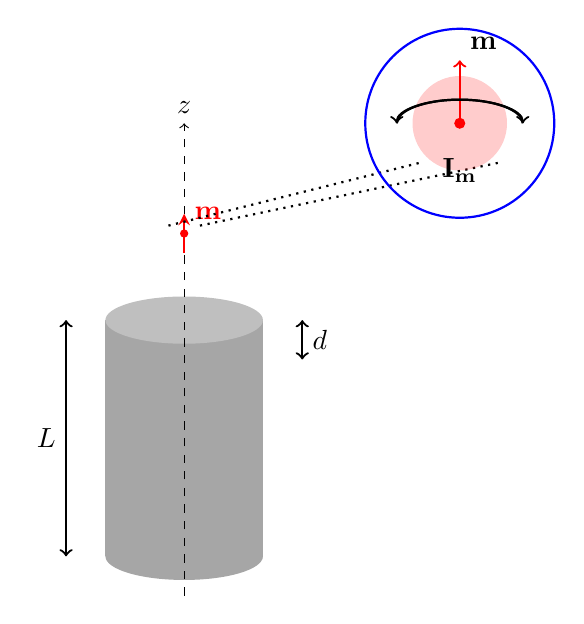
\begin{tikzpicture}
            % Cylinder
            \fill[gray!70] (-1,-3) rectangle (1,0); % Cylinder side
            \fill[gray!50] (0,0) ellipse (1 and 0.3); % Top ellipse
            \fill[gray!70] (0,-3) ellipse (1 and 0.3); % Bottom ellipse

            % Dimension L
            \draw[<->, thick] (-1.5,0) -- (-1.5,-3) node[midway,left] {\(L\)};

            % Dimension d
            \draw[<->, thick] (1.5,-0.5) -- (1.5,0) node[midway,right] {\(d\)};

            % z axis
            \draw[->, dashed] (0,-3.5) -- (0,2.5) node[above] {$z$};

            % Magnetic moment vector m
            \fill[red] (0,1.1) circle (1.5pt);
            \draw[-stealth, thick, red] (0,0.85) -- (0,1.35) node[right] {\textbf{m}};

            % Zoom lines to indicate enlargement
            \draw[dotted, thick] (0.2,1.2) -- (4,2);
            \draw[dotted, thick] (-0.2,1.2) -- (3,2);

            % Zoomed-in circle (zoom view)
            \begin{scope}[shift={(3.5,2.5)}, scale=1]
                % Outer circle for the zoomed view
                \draw[thick, blue] (0,0) circle (1.2);

                % Red shaded circular area in the background
                \fill[red, opacity=0.2] (0,0) circle (0.6);

                % Magnetic moment vector m
                \fill[red] (0,0) circle (2pt); % Central point of the magnetic moment
                \draw[->, thick, red] (0,0) -- (0,0.8) node[above right, black] {\textbf{m}};

                % Elliptical path for current I_m with directional arrows
                \draw[->, thick] (-0.8,0) arc[start angle=180, end angle=0, x radius=0.8, y radius=0.3];
                \draw[->, thick] (0.8,0) arc[start angle=0, end angle=180, x radius=0.8, y radius=0.3];

                % Label for current I_m
                \node at (0,-0.6) {\(\mathbf{I_m}\)};
            \end{scope}

        \end{tikzpicture}
    \end{center}

\end{exercício}
\begin{proof}[Resolução]
\end{proof}

\end{document}
